This chapter provides an overview and analysis of related works.
Subsequent sections introduce characteristics of satellite imagery, discuss topics of deep learning and super-resolution.
Following part of the work provides theoretical grounding for techniques used in the latter Chapters \ref{ch:scope}, \ref{ch:augmentation} and \ref{ch:sr-evaluation}.

\section{Overview of super-resolution techniques}
As mentioned in Chapter \ref{ch:introduction} super-resolution techniques can be divided into single and multi-image categories where one or many low resolution images are turned into a high-resolution one.
The latter is more advanced technique, which utilizes multiple low-resolution
images of the same scene to produce one high resolution picture.
The usual approach is to utilize multiple low--resolution images that are slightly shifted (in subpixel domain).
Data from these multiple images is merged together to produce an image of greater quality \cite{kawulok-2019-multisr}.
This approach can lead to best results in super--resolution.
In some scenarios the data fusion can lead to recreation of high resolution details that are hardly visible in any single low--resolution image.
In the case of multi-image super-resolution, better image quality comes at a cost of obtaining a series of input pictures instead of one, as it is in the single-image approach.

The simplest super-resolution approach predates deep-learning techniques and utilizes interpolation techniques for multi-image data.
Multiple low-resolution images with subdomain shifts can be used to achieve more detailed interpolation for missing values in the reconstructed high-resolution picture \cite{park-2003-sr}.
Nowadays super-resolution is mainly done with deep learning techniques which undergo a rapid development.
Deep learning based super-resolution can be divided in regard to: supervision (supervised or unsupervised learning), application domain, network architecture, learning strategy and evaluation technique \cite{wang-2019-srsurvey, bashir-2021-srreview}.

\section{Characteristics of satellite imagery}
This work centers around super--resolution technique in the sphere of satellite imagery.
As mentioned in the introduction (Chapter \ref{ch:introduction}), image enhancing can be domain-specific.
This is especially crucial when satellite photos are taken into account.
Pictures taken from aerospace devices differ substantially from normal photography.
Multi-image observation is usually favoured over single--image.
Satellites often take a series of photos of a single scene.
This puts emphasis on the multi image super--resolution techniques in the many--to--one fashion.

Another unique feature of satellite observations is the usual spectral width of the imagery.
Scientific \textit{hyper--spectral} apparatus present on satellites often take photos in a very wide spectrum that may not include frequencies of visible light.
This specific kind of image with large spectral dimension is often called a \textit{hyper--spectral cube}, because it can be represented as a three--dimensional tensor (cube) with height, width and spectral dimensions.
Spectral bands in the cube have the same width and sample adjacent parts of spectral range.
The \textit{multi-spectral} devices take pictures in multiple different bands of different wavelenghts.
Spectral bands in a multi-spectral image can contain wavelengths such as infrared, near--infrared, panchromatic\footnote{A spectral range similar to the range of traditional monochromatic grayscale photography. This range is usually highlighted because of connections with pre--digital imaging of the past century.}, radio frequencies and more.
Such images are often stored in special file formats or in a series of high bit--depth standard lossless image formats, such as PNG or TIFF.
These can take up to 13 bands  or more in different files per a single satellite photography.

One more crucial property of satellite imagery is the GSD (\textit{ground sample distance}) parameter, which denotes spatial distance between pixels of a digital image.
For example, one--meter GSD states that that location of adjacent pixels is one meter apart on the ground.
The GSD parameter determines size of objects visible in the satellite pictures.

Super-resolution for satellite imagery has been developing rapidly in recent years.
The growth of this field was accelerated by Proba-V super-resolution competition organized by the European Space Agency \cite{esa-proba-competition} .
The challenge lasted from the end of 2018 to June of 2019 (over half a year).
Architectures submitted in the competition have pushed super-resolution beyond previous baseline performance scores.
A more detailed description of the Proba dataset can be found in Section \ref{sec:probav}.

\section{Machine learning for image processing}
Both the augmentation process and the super-resolution implementations in this work are baed on machine learning---especially deep learning.
Following chapters provide an overview of these methods for image processing.

\subsection{Neural networks and deep learning}
\textit{Machine learning} is a computer science technique that solves problems by fitting algorithms to data, by optimization algorithms and statistics.
This approach contrasts with the traditional imperative problem--solving, where algorithms are designed with step--by--step attitude.
\textit{Artificial neural networks} are machine learning structures modeled after living organisms and structure of brain.
The traditional neural networks consist of layers of densely connected neurons.
Each of the neurons contains a set of inputs with connected weights.
The output of a neuron is passed through a nonlinear activation function.

Training a neural network in a supervised manner requires a set of examples bounded with ground truth labels.
The fitting process of such a network consists in adjusting the input weights.
Learning is done in steps called \textit{epochs}, during each epoch the training set is passed through the network.
The output of the network is then compared with the ground truth labels.
This is done according to a given \textit{loss function} which serves as a metric between the actual and expected output of the network.
Then the loss is used to optimize the wights via \textit{gradient descent} methods.
The gradients are computed using \textit{backpropagation} algorithm which is based on the chain rule of derivatives.
There are various loss functions and optimizers to choose from and apply according to the given problem.
In modern deep learning datasets may be too big to apply backpropagation in one pass.
For this reason, weights are usually updated using small subsets called \textit{batches}.

This kind of machine learning architecture has been initially used with manual feature extraction.
Utilization of a set of predefined convolutional filters may be an example of this approach in the domain of image processing.
A set of such filters would include basic geometric shapes.
These small filters would be convolved with the input image.
The results of such an operation would be then fed into the neural network to get the final result of image processing.
With the advancements in the machine learning area, a new kind of neural network layer was created---a \textit{convolutional layer}.
These layers consist of (one, two or even three dimensional) filters that can be convolved with the input image.
However, in  contrast to the manual feature extraction technique, these filters are adjusted in the fitting process of the network.
Elements in the filter tensor are treated like neuron weights, and they are accommodated during gradient descent.
This enables creation of much better perfoming and flexible image processing neural networks.
Convolutional layers can also be viewed as a dense layer with shared weights between groups of pixels.
This way, every pixel can be used in the fitting process without connecting every value in the image, which would result in very big and hard-to-train networks.

However, the creation of convolutional neural networks leads to increasing complexity and number of parameters in models.
This issue can be addressed by using very large datasets for the fitting process.
Nowadays, the smallest datasets for training modern neural networks contain thousands of images.
Such trainings require a lot of time and processing power; they usually must be performed using (even multiple) GPUs and may last a few days.
This combination of three factors: complex multi--layered neural networks (often with media--oriented specialized layers), very large datasets (often with many classes and objects) and utilization of expensive time and resource--consuming trainings constitute what is called \textit{deep learning}.
This kind of machine learning has proven, in the last ten years, to hold a revolutionary potential, pushing forward techniques such as image and audio processing beyond what is possible with older methods.
Modern super--resolution, which this work revolves around, is possible thanks to advancements in the deep learning.

\subsection{Encoder--decoder mechanism}
Encoder--decoder network architecture is a common pattern in generative image processing.
It is used both in data augmentation networks presented and super-resolution model utilized in Chapters \ref{ch:augmentation} and \ref{ch:sr-evaluation}.
Encoder--decoder translates input data into abstract state during encoding, then reconstructs it when decoding.
The mid--point of the architecture usually bottlenecks the information containing compressed--like data.
Convolutional interpretation of the encoder--decoder is usually used when working with images.
During the encoding process the depth of input is usually increased and spatial dimensions are shrunken.
This is achieved by subsequent usage of convolutional and pooling layers.
After encoding, the compressed data can undergo some form of processing.
For example, it can be flattened and passed through a densely connected layer, although this is rarely applied in the super--resolution, because fully--connected layers break the fully convolutional nature of a network (meaning that it cannot process images of varying spatial size).
The decoding process commonly reconstructs depth dimensions into spatial size by upsampling or transposed convolution.
The output may match the input dimension; however, it is not necessary.
In super--resolution it is common to output data of different size than the input.
Encoder--decoder architecture is appropriate for image--to--image transformations in machine learning.
The inner workings of such an architecture are shown in the figure \ref{fig:encoder-decoder}, where $ x $ and $ y $ denote input and output and $ z $ is the encoded hidden state. 
\begin{figure}
    \centering
    \documentclass[tikz]{standalone}
\usepackage[utf8]{inputenc}

\usetikzlibrary{positioning}
\usetikzlibrary{shapes.geometric}

\begin{document}
	
\tikzset{arrow/.style={-stealth}}

\begin{tikzpicture}
	\node[fill=blue!20, minimum width=0.5cm, minimum height=3.5cm] (X) at (0,0) {$\mathbf x$};
	
	\draw([xshift=0.5cm]X.north east) -- ([xshift=2.5cm,yshift=0.5cm]X.east) -- ([xshift=2.5cm,yshift=-0.5cm]X.east) -- ([xshift=0.5cm]X.south east) -- cycle; 
	\node at (1.75,0) {\textsc{Encoder}};
	
	\node[fill=blue!20, minimum width=0.5cm, minimum height=1.0cm] (Z) at (3.5cm,0) {$\mathbf z$};
	
	\draw([xshift=0.5cm]Z.north east) -- ([xshift=2.5cm,yshift=1.25cm]Z.north east) -- ([xshift=2.5cm,yshift=-1.25cm]Z.south east) -- ([xshift=0.5cm]Z.south east) -- cycle;
	\node at (5.25,0) {\textsc{Decoder}};
	
	\node[fill=blue!20, minimum width=0.5cm, minimum height=3.5cm] (Xp) at (7,0) {$\mathbf y$};
	
	\draw[arrow] (X.east) -- ([xshift=0.5cm]X.east);
	\draw[arrow] ([xshift=-0.5cm]Z.west) -- (Z.west);
	\draw[arrow] (Z.east) -- ([xshift=0.5cm]Z.east);
	\draw[arrow] ([xshift=-0.5cm]Xp.west) -- (Xp.west);
\end{tikzpicture}
\end{document}
    \caption{Schematic of encoder--decoder mechanism}
    \label{fig:encoder-decoder}
\end{figure}

Encoder--decoder mechanism is often enhanced with \textit{residual connections}.
These are often called \textit{skip connections} because they form parallel branches in networks that skip certain operations.
These skip routes are then summed with the result of an operation, resulting in additional direct flow of information during forward and direct gradient flow on the backward pass.
Residual connections applied between arms of an encoder--decoder create what is called \textit{U--Net} architecture.
In the case of super--resolution processing, the forward skips can be viewed as routes for transporting unprocessed low--frequency information.
This information can be used during the decoding step in the encoder--decoder scheme.

\subsection{Generative Adversarial Networks}
\label{sec:gans-overview}
In recent years, a new approach to training generative neural networks has emerged.
The traditional supervised learning described in the previous sections consists in providing the network with an input and comparing the generated output with a ground truth to compute loss.
The \textsc{gan}---\textit{generative adversarial network} approach requires creating two networks, a \textit{generator} and \textit{discriminator} \cite{goodfellow-2014-gans}.
The former is tasked with generating data, while the latter learns to differentiate images created by the generator from real ones.
In the \textsc{gan} scheme the discriminator learns like a traditional binary classifier---it is provided with real and generated images, which are labeled accordingly.
Then discriminator loss is computed using standard classification metrics like \textit{binary cross--entropy}.
However, the generator learns in a more unique way; it creates an output image that is fed into a discriminator.
The generator loss is calculated depending on how well it produces data that may be classified as \textit{real} by a discriminator.
If the generated image is recognized as a \textit{fake} one, it receives a big penalty in the form of a large loss.
The inner-workings of a \textsc{gan} network can be visualized in the form of a graph, as in the figure \ref{fig:gan-training}.
\begin{figure}
    \centering
    \documentclass[tikz]{standalone}
\usepackage[utf8]{inputenc}

\usetikzlibrary{positioning}
\usetikzlibrary{shapes}
\usetikzlibrary{calc}

\begin{document}
	
\tikzset{arrow/.style={-stealth}}

\begin{tikzpicture}[ampersand replacement=\&]
   	\node[text width=0.25cm] at (-2.5,0) (X) {$ \mathbf x $};		 
    \node[rectangle, rounded corners, draw, fill=blue!20, minimum height=1cm] at (0,0) (G) {\textsc{Generator}};	
    \node[rectangle, rounded corners, draw, minimum height=1cm] at (3,0) (S1) {\textsc{Sample}};
    
    \node[text width=0.5cm] at (0.75,3) (Y) {$ \mathbf y_{gt} $};		 
    \node[rectangle, rounded corners, draw, minimum height=1cm] at (3,3) (S2) {\textsc{Sample}};
    
    \node[rectangle, rounded corners, draw, fill=blue!20, minimum height=1cm] at (6,1.5) (D) {\textsc{Discriminator}};
    
    \node[text width=2cm] at (10,1.5) (O) {\textsc{Real/Fake Prediction}};
     
    \path[arrow] (X) edge (G)
    (G) edge (S1)
    (S1) edge (D.south west)
    (Y) edge (S2)
    (S2) edge (D.north west)  
    (D) edge (O)
    ;
\end{tikzpicture}

\end{document}
    \caption{Schematic of \textsc{gan} network inner--workings}
    \label{fig:gan-training}
\end{figure}

\textsc{Gan}s can have many variations, the most common type utilizes unsupervised or semi--supervised data generation.
This means that in many GANs the generator can be fed with values from proper random distribution (often called \textit{latent space}) to generate new data.
An ability to create images without direct input is a great advantage of adversarial networks.

In general, adversarial network architectures provide great generative capabilities.
For this reason, GANs are widely used for data augmentation and creation \cite{bulat-2018-supergan, sundaram-2021-gangen, shorten-2019-augmentation, perez-2017-augmentation}.
A variant of GAN architecture is later used in this work for creating super-resolution training data in Chapter \ref{ch:augmentation}.

\subsection{Measuring quality of image--generating neural networks}

Both super--resolution networks and data augmentation networks input and output images.
Quantitive evaluation of such networks require comparison of two images---the network output and the ground truth reference image.
Images are usually compared using metrics like \textit{mean absolute error}, \textit{mean square error} and \textit{peak signal to noise ratio (PSNR)}.
These calculate error between pairs of corresponding pixels in different ways.
However, these metrics may be insufficient for super--resolution related problems.
Calculating pixel--wise differences does not resemble the way humans estimate image quality.
Images of varying perceived quality can have the same \textit{PSNRs} compared to the reference image.

To measure image similarity in a more reliable way \textit{structural similarity index (SSIM)} \cite{wang-2004-ssim} was introduced.
\textit{SSIM} calculates image quality in three main components:
\begin{itemize}
	\item Average \textit{luminance}.
	\item \textit{Contrast} as standard deviation of pixels.
	\item \textit{Structure} as luminance difference divided by standard deviation.
\end{itemize}
However, these values are not calculated globally.
Instead, \textit{SSIM} values are measured using windows with pixel weights determined by Gaussian distribution.
Values of \textit{SSIM} components are combined using a compound formula.
The precise mathematical description of the SSIM metric can be found in the bibliography.
Advantages of \textit{structural similarity index} render it suitable for super--resolution related image quality evaluation.

However, modified versions of the previously mentioned traditional metrics can also prove to be useful in the image comparison, one of them being the \textit{cPSNR}.
The traditional PSNR has a potential drawback of being sensitive to bias in image brightness.
This metric equalizes average brightness of compared images before calculating standard PSNR to alleviate this problem.
The improved version of PSNR was introduced and used for scoring in the Proba-V super-resolution competition \cite{esa-proba-competition}.
Various of the mentioned metrics were in this work, in accord to specific requirements of each step in the augmentation and super--resolution training process.

\subsection{Image registration}
\label{sec:registration}
Another challenge often encountered during super--resolution training and evaluation consists in aligning image pairs correctly.
Often two images that are to be compared are slightly shifted; it is common for these dislocations to lie in sub--pixel domain.
The process of aligning two similar images is called \textit{image registration}.
Registration can be performed either with traditional or deep learning-based algorithms.
To register the sub--pixel translations, images can be upscaled before using a matching algorithm.

Registration algorithms can be divided by the applied methodology of image processing.
The first group of methods works on image features and properties.
These algorithms can detect image area characteristics like boundary regions, corners and frequency properties.
Image features can also be detected by similarity measures and image descriptors like \textit{SIFT}, \textit{SURF} and statistical properties, e.g. \textit{cross-correlation} (more detailed description of various methods can be found in \cite{jain-2015-registration}).
Pictures can also be characterized by frequency-domain based traits like \textit{phase--correlation} \cite{guizar-2008-registration}.
This method utilizes two--dimensional \textit{Fourier transform} on images.

Another branch of image registration techniques takes an advantage of modern machine-learning technologies.
These can utilize learning approaches like deep learning with similarity metrics or unsupervised trainings \cite{haskins-2020-deepregistration}.
A modified version of an image inpainting deep neural network can be used as a well-working registration algorithm \cite{deudon-2020-highresnet, zhaoyi-2018-shiftnet}.
More detailed explanation of such an approach is included in section \ref{sec:shiftnet}.

\subsection{Data augmentation in machine-learning}
Data augmentation techniques are briefly characterized in the introductory Section \ref{sec:augmentation-introduction}.
However, this field is a very wide area of research, ranging from applying simple modifications to existing samples to generating synthetic datasets \cite{kar-2019-synthetic}.
Traditional augmentation techniques include operations like zooming, resizing, shifting, flipping, rotating, distorting, adding noise, random erasing, image mixing, applying predefined filters, modifying colors and exposure.
Data augmentation is useful for preventing overfitting and training complex networks on relatively small datasets \cite{shorten-2019-augmentation}.
These operations may be application--specific.
To give an example, one should beware of distorting or flipping data containing with constrained geometry, like road signs.

The traditional augmentation techniques lead to great results; however, more modern approach based on deep learning can be used to widen data generation capabilities.
The popularization of GAN networks has led to great advancements in data generation.
Thanks to the adversarial networks entirely artificial samples can be generated \cite{sundaram-2021-gangen} even on-line during the training process \cite{bulat-2018-supergan}.

\section{Super--resolution with HighRes--net}
In recent years many super--resolution architectures have emerged due to advancements in deep learning techniques.
At the moment the state--of--the art model is RAMS (\textit{Residual Attention Multi-image Super-resolution}).
However, in this work \textit{HighRes--net} architecture is utilized.
\textit{HighRes--net}, which is few months older, achieves slightly worse results; however, it is simpler and faster to train \cite{paperswithcode-ranking}.
Because the aim of the work is to compare different data generation techniques, not the super--resolution algorithms themselves, the more manageable architecture was chosen.
A brief description of the more sophisticated architecture is also given to provide a wider context.

\subsection{Architecture overview}
\textit{HighRes--net} \cite{deudon-2020-highresnet} is a super--resolution network based on generative deep learning.
It falls into the category of \textit{multi--frame super--resolution (MFSR)} algorithms, which takes \textit{many--to--one} (or \textit{multi--image}) approach to output generation.
In MSFR systems input is a series of images, taken with a slight shift, perhaps with a small time interval.
The input series contains more information, than a single image, as a result of random displacements, noise disturbances and atmospheric conditions.
MSFR tackles the problem of aliasing in sampled data.
Low frequency parts of the image, with large geometry and little detail don't differ much between many images.
However, MSFR is crucial when enhancing small detailing.
Upscaling small details from a single image can be non--reliable due to aliasing.
Applying MSFR techniques and multiple low--resolution images fusion leads to de--aliasing information contained in the images.
\textit{HighRes--net} processing is divided into four subtasks:
\begin{enumerate}
	\item \textbf{Co--registration}, which estimates relative geometric differences between input images. These include divergences, due to shifts, rotations, deformations, etc.)
	\item \textbf{Fusion}, which combines multiple input images into a single one, that is more refined.
	\item \textbf{Up--sampling}, which upscales low into high--resolution image.
	\item \textbf{Registration--at--the--loss}, which estimates relative geometric differences of high--resolution prediction and ground truth, for more representative loss calculation. After calculating shift between super--resolution output and reference image, they are aligned using Lanczos resampling and then loss is measured.
        % TODO: ref shiftnet
	    The registration and alignment are learned by a model inspired by a \textit{ShiftNet} network architecture.
\end{enumerate}
The unique feature of \textit{HighRes--net} is that all of its parts are learned in a single fit in an end--to--end fashion.

\subsection{Super--resolution inference process}
The inference pipeline of HighRes--net is shown in the figure \ref{fig:highresnet-inference}.
The consecutive paragraphs will walk through each step in the process and explain how super--resolution is performed.
\begin{figure}
    \centering
    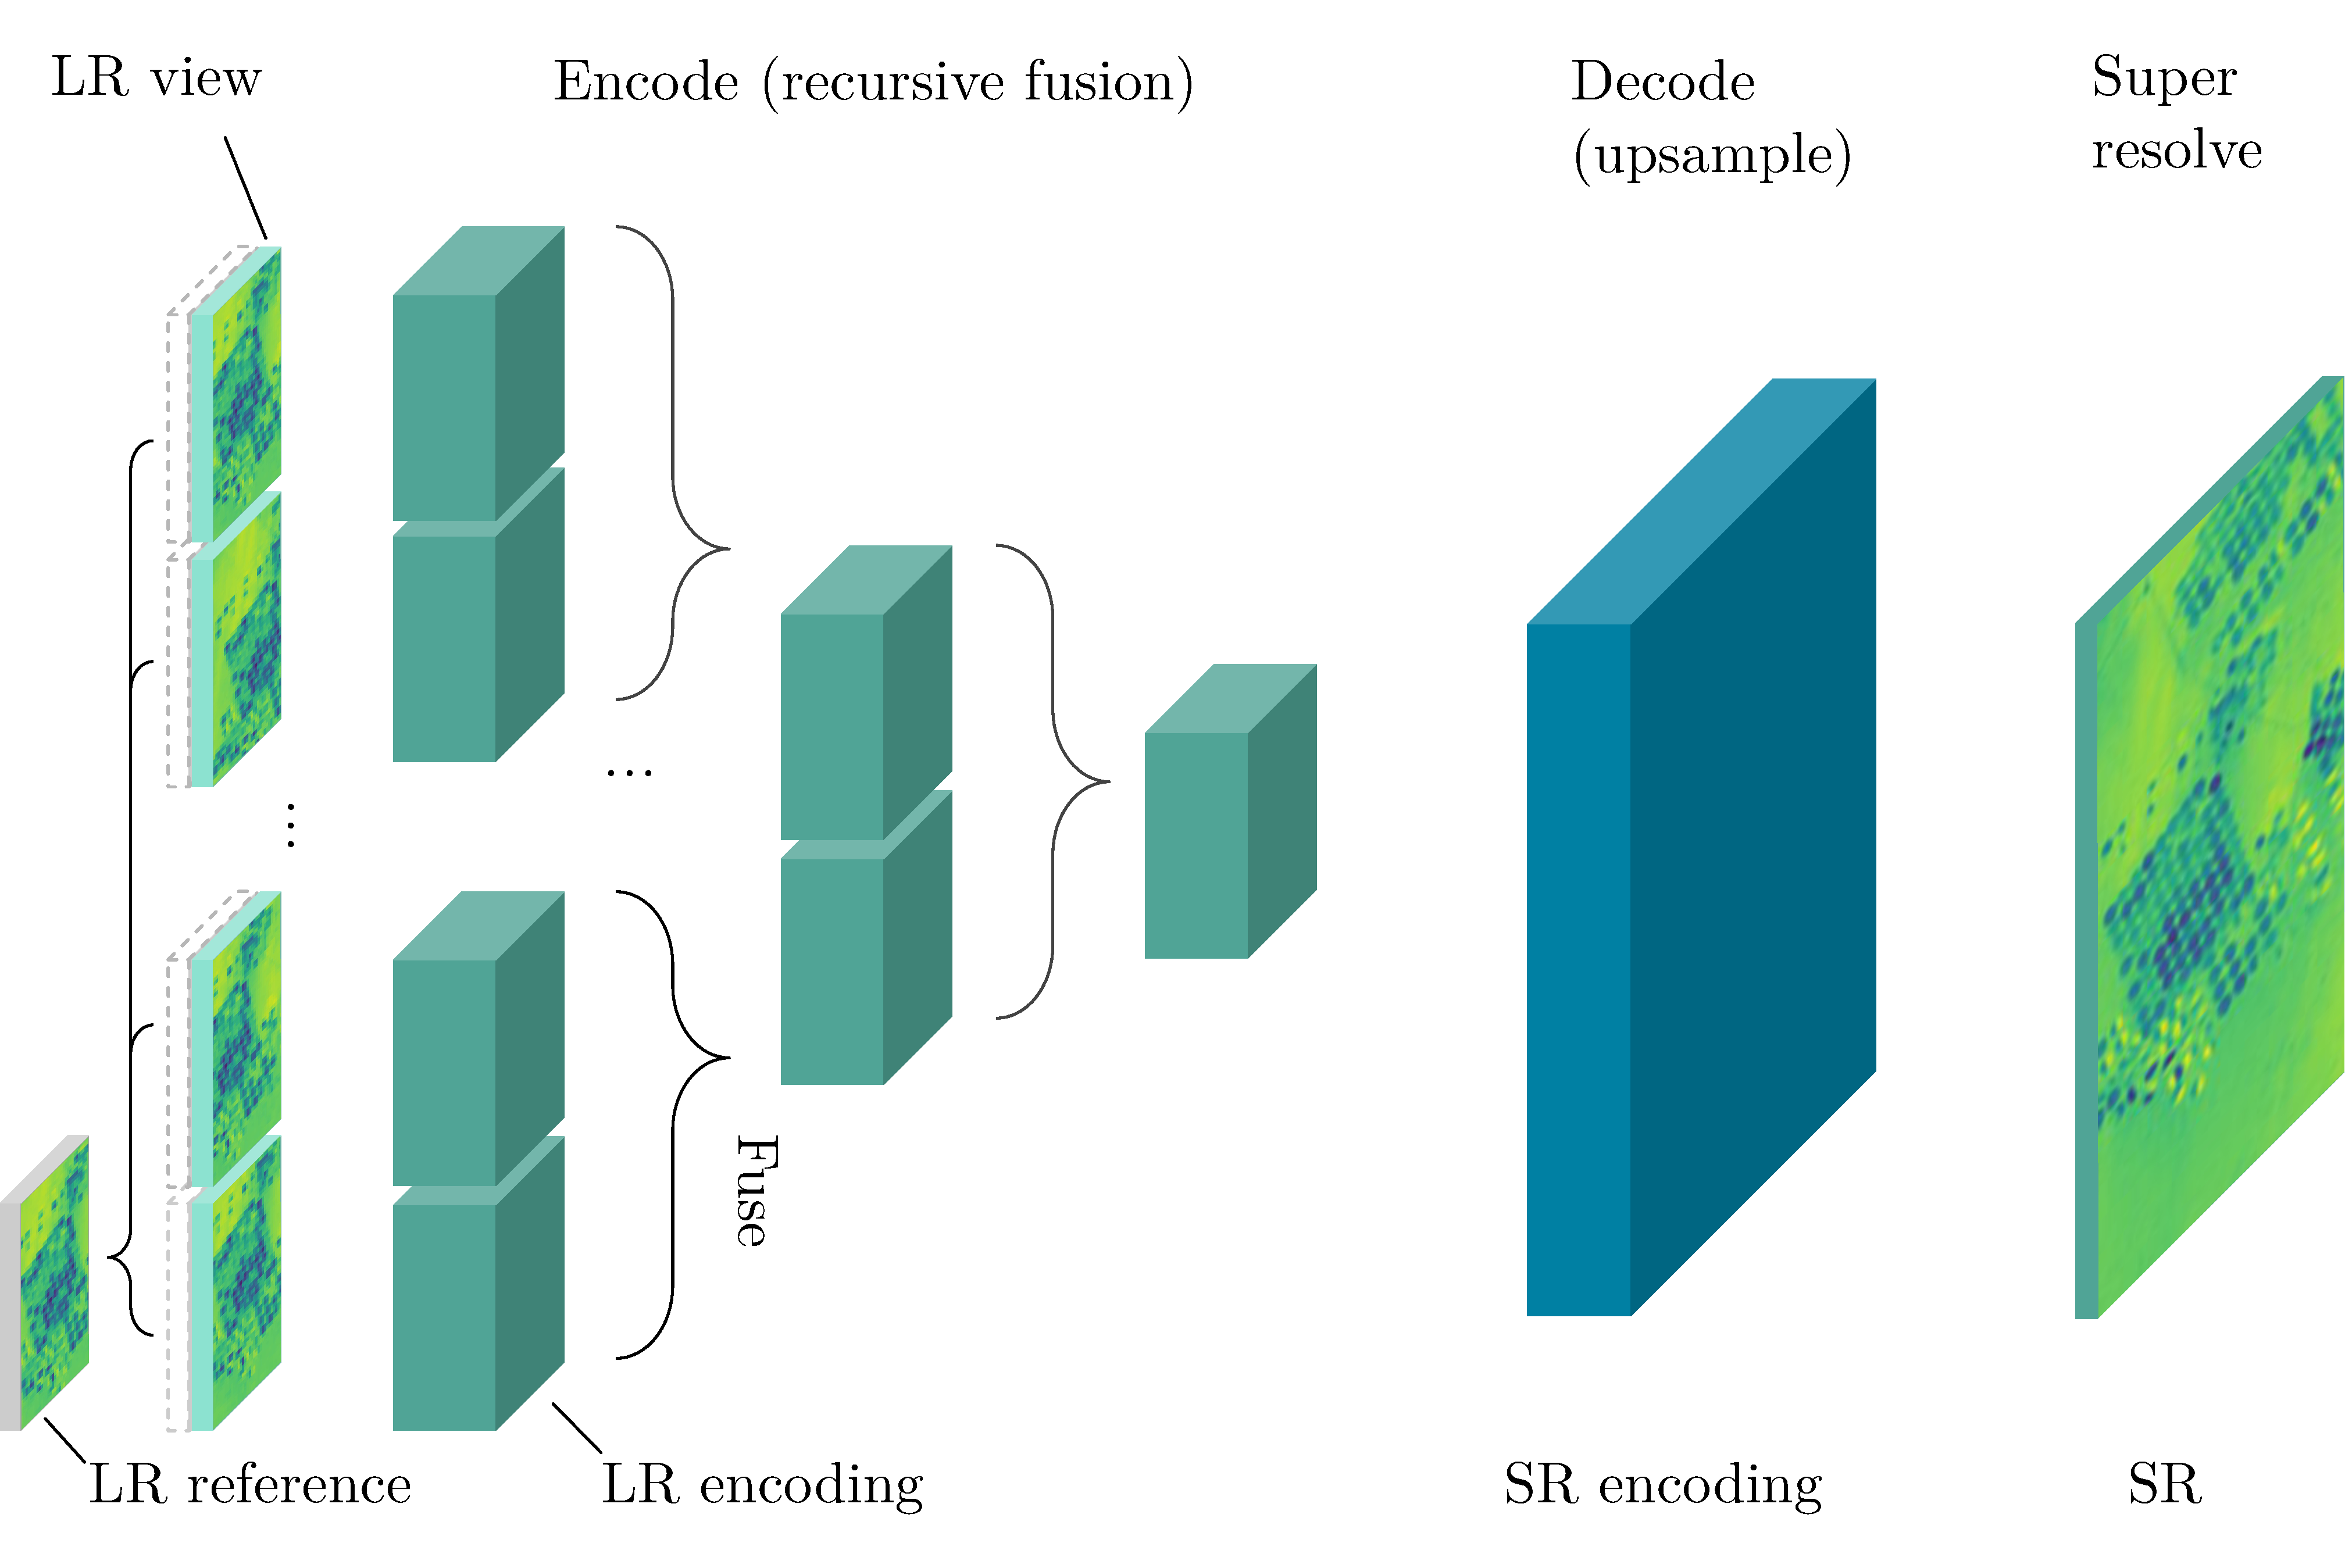
\includegraphics[width=\textwidth]{high_res_net_inference}
    \caption{Schematic of inference in \textit{HighRes--net} \cite{deudon-2020-highresnet}}
    \label{fig:highresnet-inference}
\end{figure}

The key element of \textit{HighRes--net} is achieving \textit{multi--frame super--resolution} by \textit{recursive fusion}.
Image generation is done by a neural network organized in an encoder--decoder scheme.
The input of the encoder is constructed from a series of low--resolution images.
If necessary, the input set is padded with zero--valued images to ensure that the number of low--resolution images is a power of 2, which is required by the network architecture.
For each input series, a \textit{reference image} is computed using median values of images.
Then the reference picture is paired with the input images.
Each low--resolution and reference pair is processed through an embedding function.
Embedding layers consists of a convolutional layer and two residual blocks with PReLu activations.
For input of length \textit{n}, output of the encoding consists of \textit{n} images, each convolved with the reference image.
In this scheme embedding learns to perform a process called \textit{implicit co--registration}, which is responsible for adjusting geometric differences between images in the input.
It is important to notice that the embedding block is a single instance shared between input pairs.

The next step in the \textit{HighRes--net} architecture is \textit{recursive--fusion}.
In this process output images are recursively fused together, pair by pair.
The fusion operation consists of two steps---co--registration of the input pair and the actual fusion.
The co--registration of fused images is similar to the co--registration of the input--reference pairs.
It is done by convolutional layer with PReLu activation and two residual layers.
Then the fusion itself is done, again by a combination of a convolutional layer and PReLu (this part doesn't include local residual layer).
The whole co--registration--fusion includes a residual connection.
Similarly to the embedding block, the fusion operator has a single instance that is shared for all steps of the recursion.

The last step of super--resolution process is to upscale the image by decoding the hidden state.
This is done with transposed convolutional layer with PReLu activation.
The transposition of the output of convolution makes the data grow in spatial dimensions, instead of the usual increase of depth when convolving.
The final image is constructed by applying convolution of size one, which doesn't change the size of the image.

\subsection{Registered loss calculation}
\label{sec:shiftnet}
As stated before, registration is an important part of \textit{HighRes--net} architecture.
It is especially crucial at the loss calculation step.
Without registration, the network would learn to output blurry images as a result of shift between predictions and targets.
Previous steps of \textit{HighRes--net} include an \textit{implicit co--registration}, where registration mechanisms learned by the network don't have to be necessarily based on shifts, but also other geometric distortions.
During evaluation it is desired to register image shifts explicitly, thus the \textit{registration--at--loss} differs from the registration performed during encoding and fusion.
At the final step, the sub--pixel registration is done by the \textit{ShiftNet--Lanczos} network.
\textit{ShiftNet} \cite{zhaoyi-2018-shiftnet} was introduced before \textit{HighRes--net}, in a separate research.
It was created with image inpainting via \textit{Deep Feature Rearrangement}.
Because this kind of filling in missing picture areas works by reusing and transferring existing data, it is suitable to be used as a registration mechanism.
It implements a modified \textit{U--Net} \cite{ronnenberger-2015-unet} architecture.
As mentioned in the introduction, U--Nets follow the encoder--decoder pattern with multiple residual connections.
Pairs of convolution and deconvolution layers in the contracting and expanding arms of a U--Net feature a residual connection.
The \textit{ShitNet} variant of \textit{U--Net} architecture contains an additional \textit{shift} operation for one of these residual connections.
More about \textit{ShiftNet} can be found in the publication.

\section{Other super--resolution architectures}
As mentioned, other super--resolution architectures are available, with RAMS \cite{salvetti-2020-rams} being the best performing one.
RAMS utilizes a novel technique called \textit{feature attention mechanism}, which enables the network to focus on high--frequency information that can be used to produce more detailed outputs.
This leads to overcoming main locality limitations of convolutional operations.
Mechanisms used in RAMS are specifically aimed at multi--image super--resolution of remote sensing data.
RAMS approach takes into account the nature of satellite imagery---relatively low spatial resolution and high depth and temporal resolution.
The attention mechanism works with three--dimensional convolutions to explore all possible directions.
This architecture puts emphasis on simultaneous data exploration and from spatial and temporal dimension resulting in the best quality of multi--image super--resolution.

\section{Resizing images with interpolation techniques}
Image resizing is a relevant topic in super--resolution, as a reference point and a tool for visualization.
It is useful as a visual baseline for super--resolution.
Traditional image resizing algorithms use interpolation to enable changing image dimensions; however, they do not create new details in the image.
A well--working super--resolution should recreate missing features when enhancing images.
Thus, it is expected that any super--resolution algorithm gives better results than image interpolation techniques.
In this work, image interpolation is used for comparisons during both the augmentation and super--resolution processes.

\subsubsection{Bicubic interpolation}
\textit{Bicubic interpolation} is one of the most prominent image interpolation modes.
Compared to other interpolation techniques it is regarded as the most advanced and time consuming of the commonly used solutions \cite{han-2013-interpolation} \cite{teoh-2008-inrepolation}.
This interpolation mode fills missing values by fitting third--degree polynomials between existing pixels.
The gradients of existing values are taken into account during the fitting process, so the interpolation splines' steepness matches the existing derivatives.
Bicubic interpolation is usually calculated in neighborhoods of four by four pixels.
Fitting polynomials to existing pixels may lead to \textit{overshooting} values.
This phenomenon often causes a slight increase in local contrast, which overall increases the \textit{acutance} (perceived sharpness) of an image.
Other image resizing modes operate on a simpler basis or consist in fitting simpler interpolation functions.
For this reason, bicubic is the most advanced and often best out of the common solutions.

\subsection{Other interpolation modes}
The bicubic interpolation has been chosen as a main reference point; however, there are other popular image resizing techniques that may be taken into account in comparisons.

The \textit{nearest neighbor interpolation} is the simplest out of widely used techniques.
In this approach the missing points are filled in with values of the closest existing pixels.
This technique often resolves in jagged edges and coarse details.

Another widely used approach is \textit{bilinear interpolation}.
Bilinear mode works similarly to bicubic one; however, it operates on simpler terms.
Instead of fitting polynomials it uses straightforward linear functions to find missing values.
Fot his reason, it cannot take into account image gradients and often results in less plausible outcome.
Furthermore, in contrast to the bicubic interpolation, bilinear usually operates in two by two neighborhoods.

\textit{Lanczos} is another interpolation method, with greater complexity and quality similar to bicubic.
In contrast to other techniques, it uses sinus function for interpolation.
Fitting is done using \textit{Lanczos filters} which may vary in function order and neighborhood size.

More details about various interpolation methods and function can be found in literature.


